\section{Selección y Definición del Tema de Investigación}

\subsection{Tema de Investigación}
"Desarrollo de una Herramienta de Diagnóstico Unificado para el Análisis de Seguridad y Geolocalización de Direcciones IP mediante Integración de Fuentes Abiertas en el Contexto de Ciberseguridad Colombiana"

\subsection{Título Provisional}
"Diagnóstico de Seguridad IP con Fuentes Abiertas en Colombia"

\subsection{Línea de Investigación}
Este proyecto se enmarca dentro de la línea de investigación en \textbf{Inteligencia de Amenazas Cibernéticas}, específicamente en el área de \textbf{Análisis Automatizado de Infraestructuras de Red} y \textbf{Desarrollo de Herramientas de Ciberseguridad Basadas en Fuentes Abiertas}.

\subsection{Área del Conocimiento}
\begin{itemize}
    \item \textbf{Área principal:} Ingeniería de Sistemas y Computación
    \item \textbf{Subárea:} Ciberseguridad y Redes de Computadores
    \item \textbf{Disciplina:} Inteligencia de Amenazas y Análisis de Vulnerabilidades
\end{itemize}

\section{Planteamiento del Problema}

\subsection{Contexto del Problema}

En el día a día de la ciberseguridad y el desarrollo de software, es común necesitar información detallada sobre una dirección IP. Un analista puede querer saber su ubicación geográfica, si está en una lista negra, qué puertos tiene abiertos o a qué organización pertenece.

Actualmente, esta información se encuentra dispersa en múltiples fuentes de datos, tanto gratuitas como de pago. Por ejemplo:
\begin{itemize}
    \item 	\textbf{Geolocalización:} Se obtiene de bases de datos como GeoLite2 de MaxMind.
    \item 	\textbf{Información de Infraestructura:} Se consulta en servicios de escaneo de Internet como Censys o Shodan.
    \item 	\textbf{Listas de Reputación:} Se verifica en plataformas como AbuseIPDB o listas de bloqueo (blocklists).
\end{itemize}

\subsection{Definición del Problema Principal}

El problema central es la \textbf{fragmentación de la información}. Un desarrollador o analista que necesita un perfil completo de una dirección IP debe realizar las siguientes acciones manualmente:
\begin{enumerate}
    \item Consultar la API o base de datos de geolocalización.
    \item Consultar la API de un servicio como Censys para obtener datos de puertos y servicios.
    \item Consultar una o más APIs de listas de reputación.
    \item Consolidar y correlacionar toda esta información a mano para poder tomar una decisión.
\end{enumerate}

Este proceso manual es \textbf{ineficiente, lento y propenso a errores}. Limita la capacidad de realizar análisis rápidos y automatizados, especialmente cuando se necesita evaluar un gran número de direcciones IP. Aunque existen herramientas comerciales que resuelven este problema, sus costos son a menudo prohibitivos para estudiantes, desarrolladores independientes o pequeños equipos.

\subsection{Pregunta de Investigación}

¿Es posible diseñar y desarrollar una herramienta de software que integre y unifique datos de fuentes abiertas y gratuitas (específicamente GeoLite2 y Censys a través de BigQuery) para presentar un diagnóstico de seguridad consolidado de una dirección IP, de manera eficiente y accesible?

\subsection{Justificación de la Investigación}

La creación de esta herramienta aborda directamente la ineficiencia del proceso actual. Al automatizar la recolección y presentación de datos, el proyecto ofrece una solución práctica que:
\begin{itemize}
    \item \textbf{Ahorra tiempo:} Reduce drásticamente el tiempo necesario para investigar una IP.
    \item \textbf{Centraliza la información:} Ofrece un "panel único" con los datos más relevantes.
    \item \textbf{Es accesible:} Al basarse en fuentes gratuitas (GeoLite2 y las cuotas gratuitas de BigQuery), la solución es económicamente viable para un público amplio.
    \item \textbf{Tiene un propósito educativo:} Sirve como un excelente caso de estudio sobre cómo integrar diferentes APIs y fuentes de datos en una aplicación de ciberseguridad funcional.
\end{itemize}

Este proyecto, aunque de alcance limitado a dos fuentes principales, sienta las bases para una herramienta más completa y demuestra la viabilidad de construir soluciones de ciberseguridad efectivas sin depender exclusivamente de costosas licencias comerciales.

\subsubsection{Análisis de Causas}
Con el fin de comprender de forma estructurada las raíces del problema identificado ---la \textit{fragmentación de la información de inteligencia sobre IPs en el contexto colombiano}--- se aplicó la metodología de Ishikawa (o diagrama de causa-efecto). Esta herramienta permitió clasificar las causas en cuatro grandes categorías: tecnológicas, económicas, humanas y regulatorias, lo cual facilita una visualización clara de los factores que convergen en el problema central.

\begin{figure}[H]
    \centering
    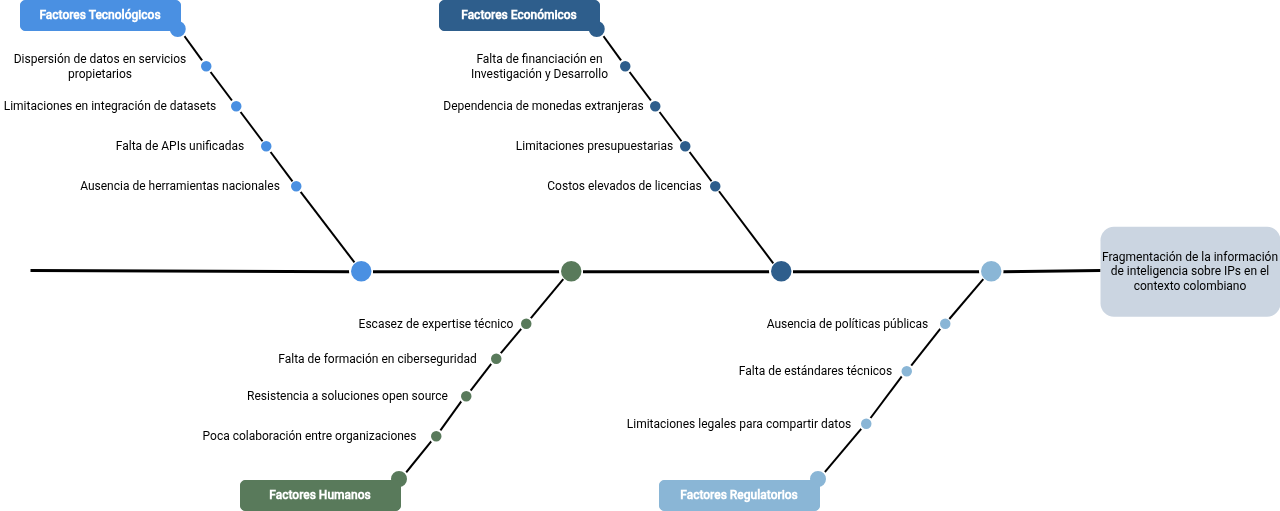
\includegraphics[width=0.95\textwidth]{sections/images/diagrama-ishikawa.png} % Ajusta la ruta y nombre del archivo
    \caption{Diagrama de Ishikawa de la fragmentación de la información de inteligencia sobre IPs}
    \label{fig:ishikawa_ips}
\end{figure}

A partir del análisis realizado, se identificaron las siguientes causas específicas:

\textbf{Factores Tecnológicos:}
\begin{itemize}
    \item Dispersión de datos de inteligencia en servicios propietarios
    \item Falta de APIs unificadas para consulta de múltiples fuentes
    \item Limitaciones técnicas en la integración de datasets heterogéneos
    \item Ausencia de herramientas nacionales especializadas
\end{itemize}

\textbf{Factores Económicos:}
\begin{itemize}
    \item Costos elevados de licencias para herramientas comerciales
    \item Limitaciones presupuestarias en organizaciones públicas y PYMES
    \item Dependencia de monedas extranjeras para servicios internacionales
    \item Falta de financiación para I+D en ciberseguridad nacional
\end{itemize}

\textbf{Factores Humanos:}
\begin{itemize}
    \item Escasez de expertise técnico especializado
    \item Falta de programas de formación en desarrollo de herramientas de ciberseguridad
    \item Resistencia al cambio hacia soluciones open source
    \item Limitada cultura de colaboración entre organizaciones
\end{itemize}

\textbf{Factores Regulatorios:}
\begin{itemize}
    \item Ausencia de políticas públicas para fomento de desarrollo tecnológico nacional
    \item Falta de estándares técnicos para herramientas de ciberseguridad
    \item Limitaciones en marcos legales para compartir información de amenazas
\end{itemize}

\subsubsection{Pronóstico}
Si persiste esta situación, se proyectan las siguientes consecuencias para el período 2025-2027:

\textbf{Impacto Operacional:}
\begin{itemize}
    \item Incremento del 40\% en tiempos de respuesta ante incidentes de seguridad
    \item Reducción del 25\% en la efectividad de detección de amenazas
    \item Aumento del 60\% en costos operativos por múltiples licencias
\end{itemize}

\textbf{Impacto Estratégico:}
\begin{itemize}
    \item Mayor dependencia de proveedores extranjeros
    \item Limitación en capacidades de soberanía digital nacional
\end{itemize}

\textbf{Impacto Económico:}
\begin{itemize}
    \item Reducción de la competitividad de organizaciones colombianas
    \item Limitación en adopción de tecnologías emergentes por riesgos de seguridad
\end{itemize}

\subsubsection{Control al Pronóstico}
Para evitar este escenario negativo, es fundamental desarrollar una solución tecnológica que:

\begin{enumerate}
    \item \textbf{Integre fuentes abiertas gratuitas} como Censys (disponible en Google BigQuery) y MaxMind GeoLite2 para proporcionar análisis comprehensivos sin costos de licenciamiento.
    \item \textbf{Implemente algoritmos de correlación avanzados} que combinen reconocimiento pasivo con geolocalización para generar evaluaciones de riesgo contextualizadas.
    \item \textbf{Proporcione interfaces intuitivas} que democraticen el acceso a capacidades avanzadas de análisis IP.
    \item \textbf{Establezca metodologías reproducibles} que puedan ser adoptadas por organizaciones con diferentes niveles de madurez tecnológica.
    \item \textbf{Genere capacidades técnicas locales} mediante documentación detallada y código abierto que facilite la transferencia de conocimiento.
\end{enumerate}